\documentclass{standalone}
\usepackage{tikz}
\usetikzlibrary{arrows,decorations.markings,calc,positioning}

% "Add arrows to a smooth tikz function"
% from http://tex.stackexchange.com/a/163695
\tikzset{
   set arrow inside/.code={\pgfqkeys{/tikz/arrow inside}{#1}},
   set arrow inside={end/.initial=>, opt/.initial=},
   /pgf/decoration/Mark/.style={
      mark/.expanded=at position #1 with
      {
         \noexpand\arrow[\pgfkeysvalueof{/tikz/arrow inside/opt}]{\pgfkeysvalueof{/tikz/arrow inside/end}}
      }
   },
   arrow inside/.style 2 args={
      set arrow inside={#1},
      postaction={
         decorate,decoration={
            markings,Mark/.list={#2}
         }
      }
   },
}

\begin{document}
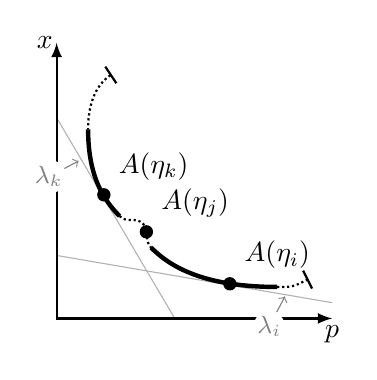
\begin{tikzpicture}

%\draw[black!5] (-0.1,-0.1) rectangle (3.6,3.6);

% simple point
%\node[circle,fill=black,inner sep=0.07cm] at (1.5,3) {};

% parameterized
%\draw[black,thick,dashed,|-|] (0.7,2.8) .. controls (0.84,2.1) and (1.12,1.12) .. (2.45,0.98);
%\node[circle,fill=black,inner sep=0.07cm] at (1.47,1.33) {};

% background slopes
\draw[black!30] (0.0,2.55) -- (1.5,0.0);
\draw[black!30] (0.0,0.8) -- (3.5,0.2);

% ok, let's have six segments!
\coordinate (cA) at (0.7,3.1);
\coordinate (cA2) at (0.4,2.9);
\coordinate (cB1) at (0.4,2.5);
\coordinate (cB) at (0.4,2.4);
\coordinate (cB2) at (0.4,1.8);
\coordinate (cC1) at (0.6,1.5);
\coordinate (cC) at (0.8,1.3);
\coordinate (cC2) at (0.9,1.2);
\coordinate (cD1) at (1.0,1.3);
\coordinate (cD) at (1.1,1.2);
\coordinate (cD2) at (1.2,1.1);
\coordinate (cE1) at (1.1,1.0);
\coordinate (cE) at (1.2,0.9);
\coordinate (cE2) at (1.4,0.7);
\coordinate (cF1) at (1.8,0.4);
\coordinate (cF) at (2.8,0.4);
\coordinate (cF2) at (3.0,0.4);
\coordinate (cG1) at (3.0,0.4);
\coordinate (cG) at (3.2,0.5);
%\node[circle,fill=blue,inner sep=0.02cm] at (cA2) {};
%\node[circle,fill=blue,inner sep=0.02cm] at (cB1) {};
%\node[circle,fill=blue,inner sep=0.02cm] at (cB2) {};
%\node[circle,fill=blue,inner sep=0.02cm] at (cC1) {};
%\node[circle,fill=blue,inner sep=0.02cm] at (cC2) {};
%\node[circle,fill=blue,inner sep=0.02cm] at (cD1) {};
%\node[circle,fill=blue,inner sep=0.02cm] at (cD2) {};
%\node[circle,fill=blue,inner sep=0.02cm] at (cE1) {};
%\node[circle,fill=blue,inner sep=0.02cm] at (cE2) {};
%\node[circle,fill=blue,inner sep=0.02cm] at (cF1) {};
%\node[circle,fill=black,inner sep=0.06cm] at (cD) {};
\draw[black,thick,densely dotted,|-]
   (cA) .. controls (cA2) and (cB1) .. (cB);
\draw[black,ultra thick,-]
   (cB) .. controls (cB2) and (cC1) .. (cC);
\draw[black,thick,densely dotted,-]
   (cC) .. controls (cC2) and (cD1) ..
   (cD) .. controls (cD2) and (cE1) .. (cE);
\draw[black,ultra thick,-]
   (cE) .. controls (cE2) and (cF1) .. (cF);
\draw[black,thick,densely dotted,-|]
   (cF) .. controls (cF2) and (cG1) .. (cG);

% at middle non-convex part
\node[circle,fill=black,inner sep=0.06cm] (Ai) at (2.2,0.44) {}; % U_i
\node[circle,fill=black,inner sep=0.06cm] (Aj) at (1.14,1.1) {}; % U_j
\node[circle,fill=black,inner sep=0.06cm] (Ak) at (0.6,1.57) {}; % U_k

%\node[circle,fill=black,inner sep=0.06cm] at (2.5,1.57) {};


%\node[circle,fill=black,inner sep=0.05cm] (a3) at (1.11,1.45) {};
\node[above right=0cm of Ai] {$A(\eta_i)$};
\node[above right=0cm of Aj] {$A(\eta_j)$};
\node[above right=0cm of Ak] {$A(\eta_k)$};

% axes
\draw[thick,latex-latex] (3.5,0) -- (0,0) -- (0,3.5);

\node[black!50,font=\small,circle,fill=white,inner sep=0pt]
   (lam1) at (2.7,-0.1) {$\lambda_i$};
\draw[black!50,->] (lam1) -- (2.9,0.28);

\node[black!50,font=\small,circle,fill=white,inner sep=0pt]
   (lam2) at (-0.1,1.8) {$\lambda_k$};
\draw[black!50,->] (lam2) -- (0.28,2.0);

% labels
%\node at (1.7,-0.25) {\small Planning Effort};
%\node[rotate=90] at (-0.25,2) {\small Execution Effort};
\node at (3.5,-0.2) {$p$};
\node at (-0.15,3.5) {$x$};

\end{tikzpicture}
\end{document}
